\documentclass[14pt]{extreport}
\usepackage{cmap}
\usepackage[utf8]{inputenc}
\usepackage[english,ukrainian]{babel}
\usepackage{graphicx}
\usepackage{geometry}
\usepackage{listings}
\usepackage{amsmath}
\usepackage{float}
\usepackage{array}
\geometry{
	a4paper,
	left=20mm,
	right=20mm,
	top=20mm,
	bottom=20mm
}
\lstset{
	language=bash,
	tabsize=4,
	breaklines,
	keepspaces,
	showstringspaces=false,
}
\graphicspath{ {./pictures} }
\setlength{\parindent}{4em}

\newcommand\subject{Аналіз вимог до програмного забезпечення}
\newcommand\lecturer{професор кафедри ПЗ\\Грицюк Ю.І.}
\newcommand\teacher{асистент кафедри ПЗ\\Масюкевич В.В.}
\newcommand\mygroup{ПЗ-32}
\newcommand\lab{2}
\newcommand\theme{Специфікація вимог до нового програмного забезпечення для обраної
	предметної області}
\newcommand\purpose{Розробити специфікацію вимог та оформити її згідно поданого
	нижче зразка}

\begin{document}
\begin{normalsize}
	\begin{titlepage}
		\thispagestyle{empty}
		\begin{center}
			\textbf{МІНІСТЕРСТВО ОСВІТИ І НАУКИ УКРАЇНИ\\
				НАЦІОНАЛЬНИЙ УНІВЕРСИТЕТ "ЛЬВІВСЬКА ПОЛІТЕХНІКА"}
		\end{center}
		\begin{flushright}
			Інститут \textbf{КНІТ}\\
			Кафедра \textbf{ПЗ}
		\end{flushright}
		\vspace{140pt}
		\begin{center}
			\textbf{ЗВІТ}\\
			\vspace{10pt}
			До лабораторної роботи № \lab\\
			\textbf{На тему}: “\textit{\theme}”\\
			\textbf{З дисципліни}: “\subject”
		\end{center}
		\vspace{40pt}
		\begin{flushright}
			
			\textbf{Лектор}:\\
			\lecturer\\
			\vspace{10pt}
			\textbf{Виконав}:\\
			
			студент групи \mygroup\\
			Коваленко Д.М.\\
			\vspace{10pt}
			\textbf{Прийняв}:\\
			
			\teacher\\
			
			\vspace{28pt}
			«\rule{1cm}{0.15mm}» \rule{1.5cm}{0.15mm} 2023 р.\\
			$\sum$ = \rule{1cm}{0.15mm}……………\\
			
		\end{flushright}
		\vspace{\fill}
		\begin{center}
			\textbf{Львів — 2023}
		\end{center}
	\end{titlepage}
		
	\begin{description}
		\item[Тема.] \theme.
		\item[Мета.] \purpose.
	\end{description}

	\section*{Лабораторне завдання}
	\begin{enumerate}
		\item Розробити специфікацію вимог для програмного продукту з предметної області система для роботи компанії з регулярних перевезень пасажирів.
	\end{enumerate}
	
	\section*{Хід роботи}
	\section*{Вступ}
	\subsection*{Призначення, мета}
	Розробка програмного продукту для оптимізації та автоматизації процесів регулярних перевезень пасажирів компанією з метою забезпечення ефективного управління розкладами, маршрутами, бронюваннями та обліком пасажирських перевезень. Створення програмної системи, яка дозволить компанії з регулярних перевезень пасажирів збільшити продуктивність та точність управління перевезеннями, зменшити витрати на ресурси та покращити задоволеність клієнтів шляхом надання зручних інструментів для реєстрації бронювань, моніторингу автопарку та статистичного аналізу даних.
	
	\section*{Загальний опис}
	\subsection*{Перспективи продукту}
	\begin{itemize}
		\item Можливість застосування програмного продукту не лише для регулярних перевезень пасажирів, але і для інших видів транспорту та логістичних компаній.
		\item Потенціал для інтеграції з системами розрахунку тарифів, електронного квиткування та аналізу даних, що допоможе компанії ще більше підвищити свою конкурентоспроможність на ринку та забезпечити розвиток бізнесу у майбутньому.
		\item Можливість впровадження продукту на міжнародному рівні для розширення географії обслуговування та залучення нових клієнтів.
	\end{itemize}
	\subsection*{Характеристики продукту}
	\begin{itemize}
		\item Програмний продукт дозволяє користувачам бронювати місця на рейсах, переглядати розклади, а також керувати рейсами і розкладами.
		\item Система підтримує обробку платежів, виставлення рахунків і ведення фінансового обліку для компанії.
		\item Програмний продукт може використовувати GPS-технологію та інтерактивні карти для відстеження рейсів, навігації для водіїв та надання користувачам точних інформаційних послуг.
		\item Система дозволяє взаємодіяти з водіями, включаючи надання їм інформації про рейси і пасажирів, а також ведення обліку автомобілів.
		\item Програмний продукт дозволяє генерувати найефективніші варіанти маршрутів та рокзладів.
		\item Система надає можливість створювати звіти і проводити аналітику даних про рейси, пасажирів і фінанси компанії.
	\end{itemize}
	
	\subsection*{Класи користувачів та їхні характеристики}
	\begin{itemize}
		\item Адміністратори системи: Мають повний доступ до управління системою, включаючи налаштування, додавання нових рейсів, керування пасажирами і водіями, а також створення звітів. Мають високий рівень технічної експертизи.
		\item Водії: Використовують систему для отримання інформації про рейси та навігації. Важливо, щоб система була інтуїтивно зрозумілою і простою у використанні.
		\item Пасажири: Пасажири використовують систему для бронювання місць, оплати, отримання квитків та отримання інформації про рейси. Важливо, щоб система була зручною та безпечною для користувачів.
	\end{itemize}
	
	\subsection*{Середовище функціонування}
	\begin{itemize}
		\item     Апаратна платформа: Сервери, комп'ютери адміністраторів і менеджерів, мобільні смартфони і планшети.
		\item Операційні системи: Linux, Windows/macOS, Android/iOS для мобільних пристроїв.
		\item Бази даних: PostgreSQL для зберігання даних про рейси і фінанси.
		\item Веб-сервери: Nginx для веб-інтерфейсу.
		\item Інші компоненти: Поштові сервери, системи моніторингу та журналювання.
		\item Інтеграція: Платіжні системи, можлива інтеграція з системами геолокації.
	\end{itemize}
	
	\subsection*{Обмеження проектування та реалізації}
	\begin{itemize}
		\item Врахування законодавчих вимог та правил щодо перевезення пасажирів, включаючи облік фінансових операцій та захист особистих даних.
		\item Використання певних технологій, фреймворків та інструментів для розробки програмного продукту може бути обмеженим на основі ресурсів і фахівців, доступних для проекту.
		\item Інтеграція з іншими системами компанії, такими як бухгалтерська програма, платіжні шлюзи або системи відстеження геолокації, може вимагати створення інтерфейсів та взаємодії з іншими додатками.
	\end{itemize}
	\subsection*{Документація користувача}
	\begin{itemize}
		\item Швидка інформація в програмі для користувачів.
		\item Часті запитання і відповіді.
		\item Контактна інформація для підтримки.
		\item Ліцензійна угода.
		\item Інформація про оновлення та зміни у програмі.
	\end{itemize}
	
	\subsection*{Припущення та залежності}
	\begin{itemize}
		\item Припускається, що користувачі будуть мати постійний доступ до Інтернету для використання програмного продукту.
		\item Вимоги можуть залежати від доступності і стабільності зовнішніх сервісів, таких як системи оплати або послуги геолокації.
		\item Вимоги можуть змінюватися в залежності від змін у відповідних законодавчих та регуляторних вимогах, наприклад, щодо обробки особистих даних користувачів.
	\end{itemize}
	
	\section*{Характеристики системи}
	
	\subsection*{Онлайн-бронювання квитків} 
	Ця характеристика дозволяє користувачам онлайн бронювати квитки на рейси. Має високий пріоритет і важливу функціональність для системи.
	
	\textbf{\textit{Послідовність дія/відгук:}}
	\begin{itemize}
		\item Користувач обирає рейс та кількість квитків.
		\item Система перевіряє доступність місць та ціни.
		\item Користувач вводить інформацію про пасажирів і обирає спосіб оплати.
		\item Система підтверджує бронювання та виділяє квитки.
	\end{itemize}
	
	\textbf{\textit{Функціональні вимоги:}}
	\begin{itemize}
		\item REQ-1: Система повинна відображати список доступних рейсів та їхню інформацію.
		\item REQ-2: Користувач повинен мати можливість обрати кількість квитків.
		\item REQ-3: Система повинна перевіряти доступність місць на вибраних рейсах.
		\item REQ-4: Користувач повинен ввести інформацію про пасажирів, включаючи імена та контактні дані.
		\item REQ-5: Система повинна обробляти різні способи оплати, такі як кредитні картки та електронні гроші.
		\item REQ-6: Система повинна підтверджувати бронювання та генерувати квитки для користувача.
	\end{itemize}
	
	\subsection*{Відстеження рейсів} 
	Ця характеристика дозволяє користувачам відстежувати рейси, перевіряти їхню поточну позицію, час відправлення та прибуття. Середній пріоритет.
	
	\textbf{\textit{Послідовність дія/відгук:}}
	\begin{itemize}
		\item Користувач вводить номер рейсу або маршрут.
		\item Система відображає інформацію про рейс, включаючи поточну позицію на мапі, час вильоту та прибуття.
	\end{itemize}
	
	\textbf{\textit{Функціональні вимоги:}}
	\begin{itemize}
		\item REQ-7: Система повинна мати можливість приймати номери рейсів або маршрути для пошуку.
		\item REQ-8: Система повинна надавати поточну інформацію про рейс, включаючи графік та позицію на мапі.
	\end{itemize}

	\subsection*{Реєстрація користувачів} 
	Ця характеристика дозволяє користувачам створювати облікові записи та зберігати інформацію про себе. Високий пріоритет.
	
	\textbf{\textit{Послідовність дія/відгук:}}
	\begin{itemize}
		\item Користувач вводить особисті дані, електронну адресу та пароль для створення облікового запису.
		\item Система перевіряє дані та підтверджує реєстрацію.
	\end{itemize}
	
	\textbf{\textit{Функціональні вимоги:}}
	\begin{itemize}
		\item REQ-9: Система повинна забезпечувати можливість реєстрації нових користувачів.
		\item REQ-10: Система повинна зберігати особисту інформацію користувача, включаючи ім'я, адресу та контактні дані.
		\item REQ-11: Система повинна забезпечувати автентифікацію зареєстрованих користувачів під час входу в систему.
	\end{itemize}
	
	\section*{Вимоги зовнішніх інтерфейсів}
	\subsection*{Користувацькі інтерфейси}
	Користувацькі інтерфейси для системи регулярних перевезень пасажирів включають веб-інтерфейс для бронювання квитків, мобільний додаток для відстеження рейсів та панель адміністратора для керування рейсами.
	
	\begin{figure}[H]
		\centering
		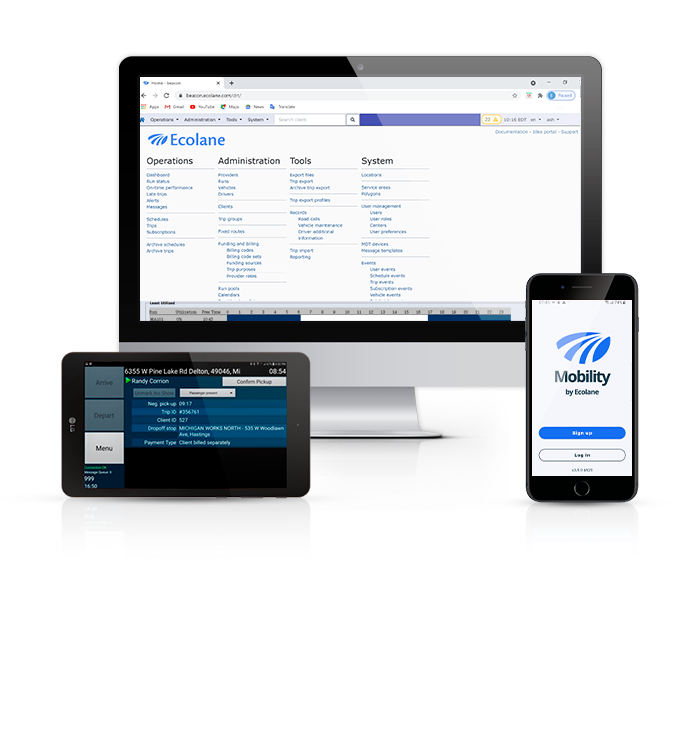
\includegraphics[trim={0 8cm 0 2cm},clip,scale=0.7]{1}
		\caption{Приклад інтерфейсу користувача}
	\end{figure}
	
	\subsection*{Апаратні інтерфейси}
	Інтерфейс для зчитування квитків:
	\begin{itemize}
		\item Типи підтримуваних пристроїв: QR-код-сканери, штрихкод-считувачі.
		\item Природа даних: Квитки з кодами.
		\item Керуючі взаємодії: Сканування та передача інформації про квиток у систему.
	\end{itemize}
	
	\subsection*{Програмні інтерфейси}
	База даних:
	\begin{itemize}
		\item PostgreSQL для зберігання інформації про рейси, бронювання та користувачів.
		\item SQL-запити для взаємодії з базою даних.
	\end{itemize}
	
	\subsection*{Комунікаційні інтерфейси}
	\begin{enumerate}
		\item Електронна пошта:\begin{itemize}
			\item Електронні листи для сповіщень та підтверджень.
			\item SMTP для відправлення повідомлень.
		\end{itemize}
		\item Мережеві протоколи: \begin{itemize}
			\item HTTP та HTTPS для взаємодії з веб-сервером.
			\item Шифрування даних через HTTPS.
		\end{itemize}
		\item Електронні форми: \begin{itemize}
			\item Веб-форми для введення та надсилання даних.
			\item HTTP або HTTPS для обробки форм на веб-сайті.
		\end{itemize}
	\end{enumerate}

	\section*{Інші не функціональні вимоги}
	\subsection*{Вимоги продуктивності}
	\begin{itemize}
		\item Продукт повинен надавати відповіді на запити користувачів у максимально прийнятний час, не перевищуючи 2 секунди для більшості операцій.
		\item Продукт повинен бути здатний обробляти і обслуговувати велику кількість одночасних користувачів без зниження продуктивності.
	\end{itemize}
	
	\subsection*{Вимоги надійності}
	\begin{itemize}
		\item Продукт повинен автоматично створювати резервні копії даних, щоб запобігти можливим втратам в інформації.
		\item Продукт повинен мати можливість відновлення після відмови системи та повернення до робочого стану.
	\end{itemize}
	
	\subsection*{Вимоги безпеки}
	\begin{itemize}
		\item Продукт повинен вимагати аутентифікації користувачів перед наданням доступу до особистих даних та функцій.
		\item Продукт повинен застосовувати шифрування для захисту конфіденційної інформації під час передачі та зберігання.
	\end{itemize}
	
	\subsection*{Атрибути якості програмного продукту}
	\begin{itemize}
		\item Продукт повинен бути гнучким і здатним адаптуватися до змін в вимогах користувачів та бізнес-процесів.
		\item Продукт повинен бути стійким до помилок та виключень, та має мінімізувати можливість відмови під час роботи.
		\item Продукт повинен бути протестований для виявлення та виправлення помилок перед випуском.
	\end{itemize}
	
	\section*{Інші вимоги}
	\subsection*{Додаток A: Словник}
	\begin{itemize}
		\item SMTP – Simple Mail Transfer Protocol.
		\item HTTPS – Hyper-Text Transfer Protocol Secure;
	\end{itemize}

	\section*{Висновок}
	Під час виконання лабораторної роботи я ознайомився з визначенням специфікації вимог для
	нового програмного продукту з предметної області "Система для роботи компанії з регулярних перевезень пасажирів". Завдяки цьому я навчився формулювати конкретні вимоги та доступно їх
	описувати.
	
\end{normalsize}
\end{document}
